\documentclass[12pt]{article}
\usepackage[utf8]{inputenc}
\usepackage[T1]{fontenc}
\usepackage{fontspec}
\setmainfont{Times New Roman}
\newfontfamily\hackfont{Hack}
\usepackage{titlesec}
\usepackage{fancyhdr}
\usepackage{listings}
\usepackage{xcolor}
\usepackage{graphicx}
\usepackage{wrapfig}
\usepackage{longtable}
\usepackage{caption}
\usepackage{hyperref}
\usepackage{setspace}
\usepackage{geometry}
\geometry{a4paper, margin=1in}
\hypersetup{colorlinks=true, linkcolor=blue, urlcolor=blue}
\renewcommand{\contentsname}{Table of Contents}

\begin{document}

% ---------------- COVER PAGE ----------------

\begin{titlepage}
\begin{center}
    
\includegraphics[width=0.35\textwidth]{assets/logo.png} \\
    \vspace{0.5cm}
    \textbf{\Huge \textcolor{cyan}{NOTRE DAME} \textcolor{cyan}{UNIVERSITY}} \\
    \vspace{0.5cm}
    \textbf{\Huge \textcolor{orange}{BANGLADESH}} \\

    \vspace{0.9cm}
    \textbf{\Huge \underline{Computer Graphics Project Proposal}} \\

    \vspace{1.5em}
    \begin{flushleft}
    	\textbf{\Large Course Code: CSE-4204} \\
		\vspace{0.3cm}
        \textbf{\Large Course Title: Computer Graphics Lab} \\
        \vspace{0.3cm}
        \textbf{\Large Project Topic: Egg Drop Game using Glut} \\
    \end{flushleft}

    \vspace{1em}
    \begin{flushleft}
        \textbf{\Huge \textcolor{blue}{Submitted by:}} \\
        \vspace{0.3cm}
        \textbf{\Large Name: Istiak Alam} \\
        \vspace{0.3cm}
        \textbf{\Large ID: 0692230005101005} \\
        \vspace{0.3cm}
        \textbf{\Large Name: Tanvir Hossain Ratul} \\
        \vspace{0.3cm}
        \textbf{\Large ID: 0692230005101004} \\
		\vspace{0.3cm}
        \textbf{\Large Batch: CSE-20} \\
        \vspace{0.5cm}
        \textbf{\Large Submission Date: }{\Large \textbf{\today}\par}
    \end{flushleft}

    \vfill
    \begin{flushleft}
        \textbf{\Huge \textcolor{blue}{Submitted to:}} \\
        \vspace{0.3cm}
        \textbf{\Large Humayara Binte Rashid} \\
        \vspace{0.3cm}
        \textbf{\Large Lecturer, Dept. of CSE} \\
        \vspace{0.3cm}
        \textbf{\Large Notre Dame University Bangladesh}
    \end{flushleft}

\end{center}
\end{titlepage}

% ---------------- TOC ----------------

\rfoot{\thepage}
\tableofcontents
\thispagestyle{empty}
\clearpage

\pagenumbering{arabic}
\pagestyle{fancy}
\fancyhf{}
\rhead{Computer Graphics Lab}
\lhead{Project Proposal}

% ---------------- MAIN CONTENT ----------------

\section{Project Proposal Description}

\subsection{Project Title}
\begin{center}
\textbf{"Egg Drop Saga" - Game}
\end{center}

\subsection{Introduction}

Computer graphics plays an important role in modern software applications, particularly in the development of interactive games and visual simulations. In this project, we will propose the development of a simple yet engaging 2D game titled \textit{Egg Drop Saga Game}. The game will be developed using the C++ programming language along with the OpenGL graphics library and the GLUT toolkit for rendering graphics and handling user input.\\
The objective of this proposed game will be to create an interactive environment where a player will control a bucket to catch eggs dropped by a chicken positioned at the top of the screen. The player will need to move the bucket left or right to successfully catch falling eggs while avoiding missed eggs.

\subsection{Objectives}

The main objectives of this proposed project will be:

\begin{itemize}
\item To design and implement a 2D interactive game using OpenGL.
\item To demonstrate the use of computer graphics primitives such as shapes, colors, and transformations.
\item To implement animation techniques for moving objects within the game.
\item To apply collision detection between game objects.
\item To create a simple but engaging user experience.
\end{itemize}

\subsection{Project Overview}

The proposed game environment will consist of three main graphical elements:

\begin{itemize}
\item \textbf{Chicken}: Positioned at the top of the screen, the chicken will periodically lay eggs.
\item \textbf{Egg}: Eggs will fall from the chicken toward the bottom of the screen at a certain speed.
\item \textbf{Bucket}: This object will be controlled by the player to catch the falling eggs.\\
\end{itemize}
The player will use keyboard input (left and right arrow keys) to move the bucket horizontally across the screen. If the bucket successfully catches an egg, the player will receive a score point. If the egg reaches the ground without being caught, the player may lose a life or scoring opportunity.

% ---------------- GRAPH SECTION ----------------

\section{Graphical Analysis}

This section will present graphical analysis related to the expected performance or behavior of the Egg Catching Game. The graph will illustrate important aspects such as gameplay performance, score progression, or object movement patterns during gameplay.

\subsection{Graph Representation}

The following figure will represent the graphical model used in this proposed project.

\begin{figure}[h]
    \centering
    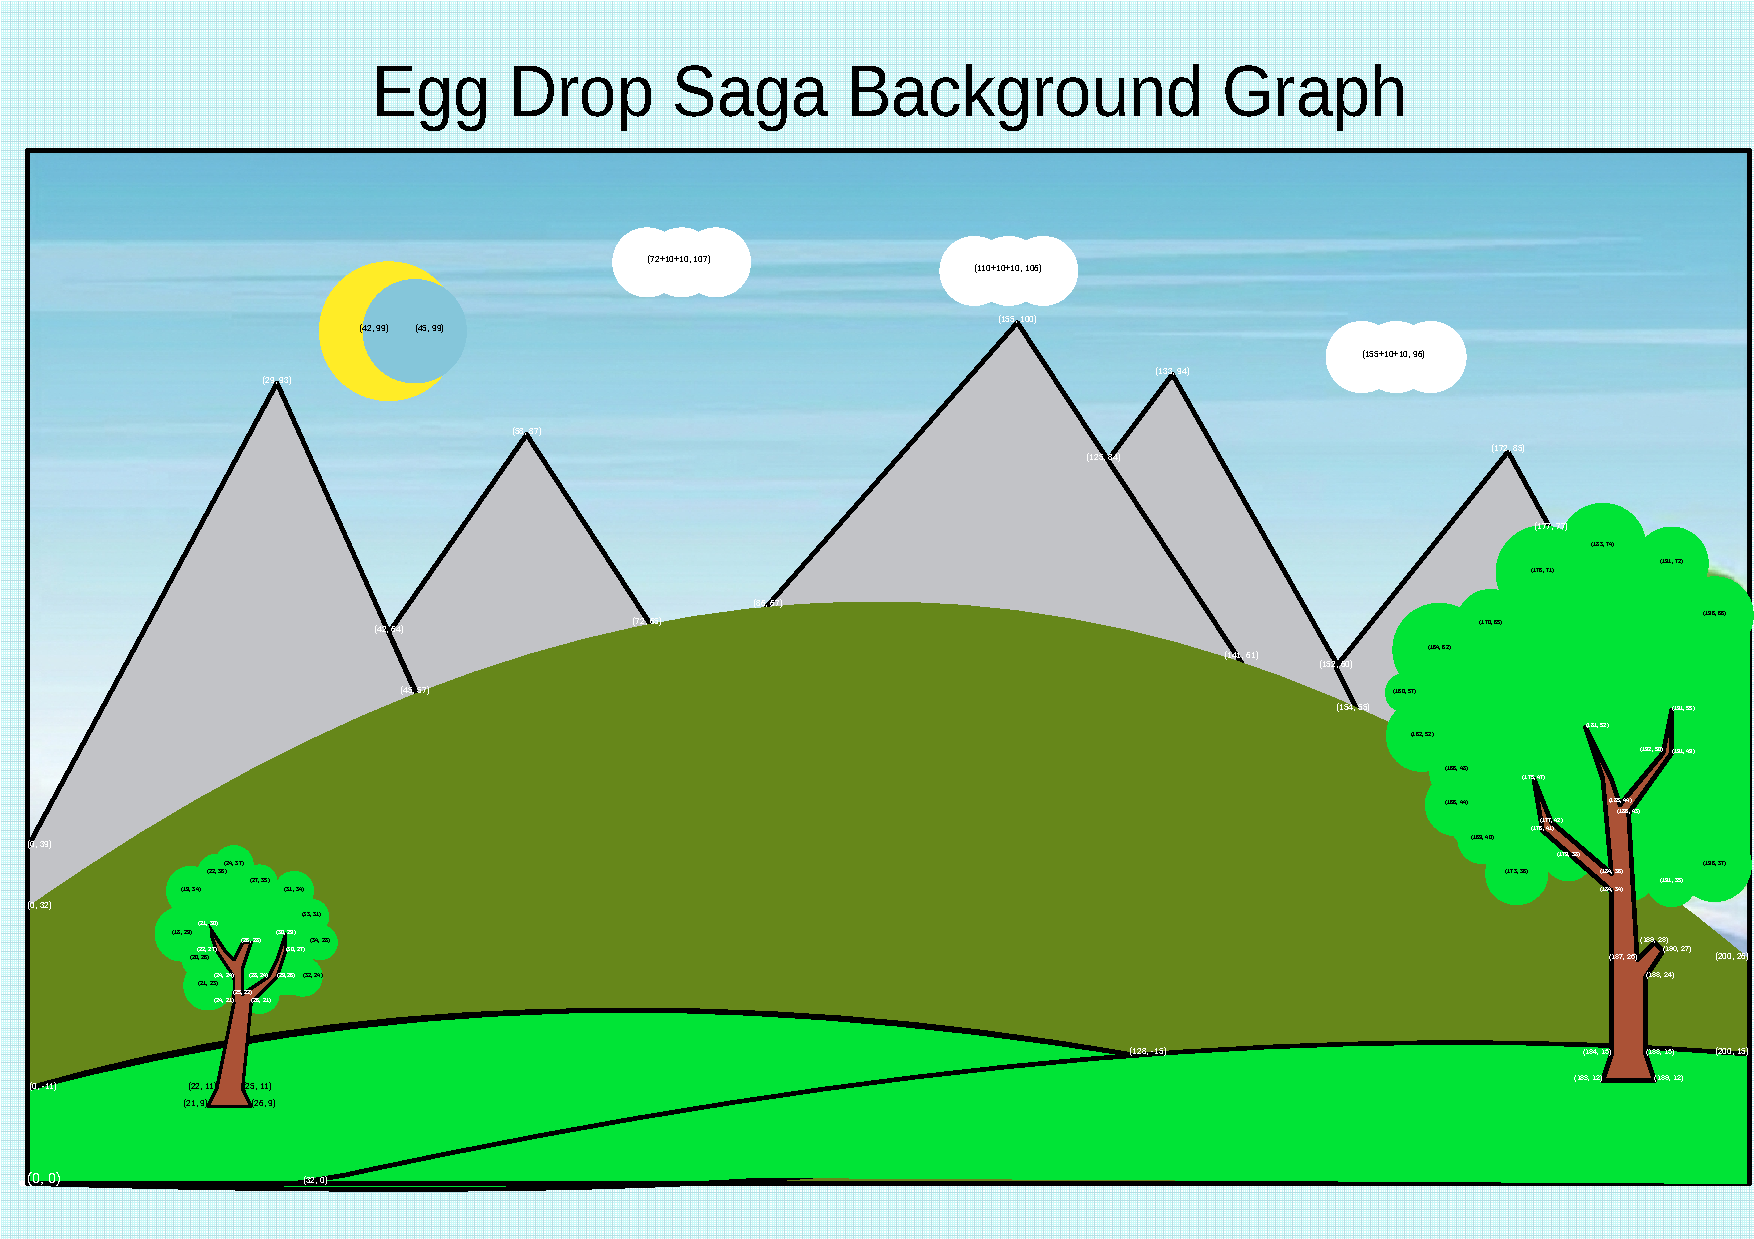
\includegraphics[width=1\textwidth]{assets/graph.pdf}
    \caption{Target Background Graph of the Proposed Egg Drop Saga Game}
\end{figure}

\subsection{Graph Source}

The graph used in this proposal can be accessed from the following resources:

\begin{itemize}
    \item PDF File: \href{https://github.com/Istiaq-Alam/Egg-Drop-Saga/blob/main/Documentation/assets/graph.pdf}{Open Graph PDF}
    \item Online Link: \href{https://virtual-graph-paper.com/ZDNjOTYyYmUxY2Nj}{Graph Source Link}
\end{itemize}

\subsection{Graph Description}

The graph will demonstrate the relationship between different gameplay parameters such as time, score, or egg spawn rate. It will help in analyzing how the game may behave during execution and will provide insights into gameplay dynamics and expected performance.

% ---------------- GAME ASSETS ----------------

\section{Game Assets}

This section will present the graphical assets that will be used in the development of the Egg Drop Saga Game. These assets will represent the main visual components of the game and will help create an engaging gameplay environment.

\subsection{Chicken Design}

The chicken will be positioned at the top of the game screen and will periodically lay eggs. To improve the visual appearance of the game, a simple animation will be implemented to simulate the chicken's movement while laying eggs.

\begin{figure}[!h]
    \centering
    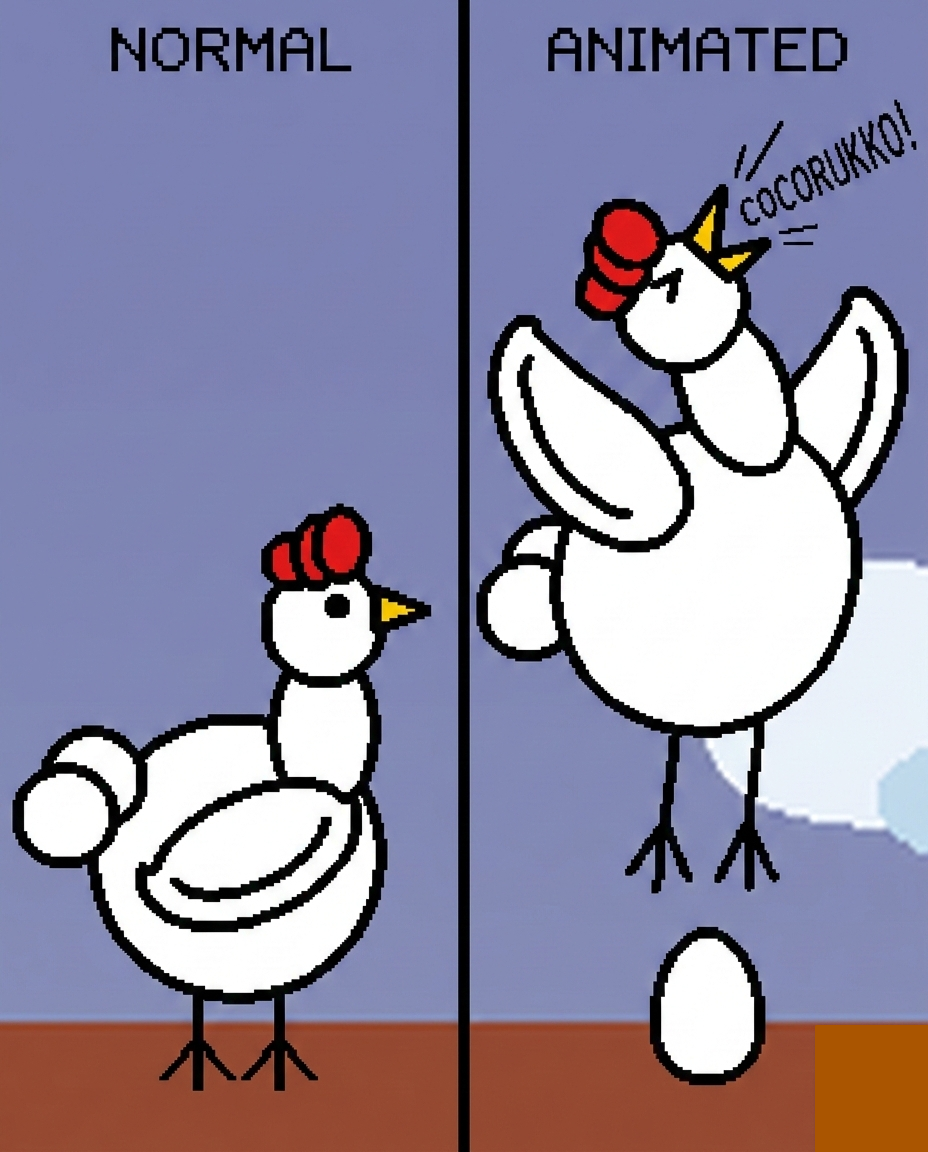
\includegraphics[width=0.35\textwidth]{assets/animated chicken.png}
    \caption{Proposed Chicken Animation}
\end{figure}

\subsection{Bucket Design}

The bucket will be the primary player-controlled object in the game. The player will move the bucket horizontally across the screen to catch falling eggs.

\begin{figure}[!h]
    \centering
    
\includegraphics[width=0.35\textwidth]{assets/Bucket.png}
    \caption{Proposed Bucket Design}
\end{figure}

\subsection{Egg Design}

The egg will be the main falling object generated by the chicken. The player will attempt to catch these eggs using the bucket in order to score points.

\begin{figure}[!h]
    \centering
    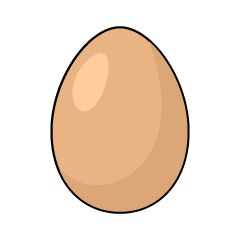
\includegraphics[width=0.35\textwidth]{assets/Egg.png}
    \caption{Proposed Egg Design}
\end{figure}

% ---------------- IMPLEMENTATION ----------------

\section{Proposed Implementation}

The project will use OpenGL primitives such as:

\begin{itemize}
\item \textbf{GL\_TRIANGLE\_FAN} for drawing circular shapes like eggs and the chicken body.
\item \textbf{GL\_QUADS} for drawing the bucket.
\item Basic color shading to represent different game objects.
\end{itemize}

Animation will be implemented through continuous screen updates using the rendering loop. The egg's vertical position will be updated over time to simulate gravity and falling motion.

\subsection{Collision Detection}

A collision detection mechanism will be implemented to determine when an egg intersects with the bucket. This will be achieved using a simple bounding box or positional comparison between the coordinates of the egg and the bucket. When a collision occurs, the egg will be considered caught and the player's score will be updated.

\subsection{Game Mechanics}

The gameplay will include the following mechanics:

\begin{itemize}
\item Eggs will be generated periodically at the chicken's position.
\item Eggs will fall downward with a constant speed.
\item The player will move the bucket horizontally to catch eggs.
\item If an egg collides with the bucket, it will be removed and the score will increase.
\item If the egg reaches the bottom of the screen, it will be considered missed.
\end{itemize}

\subsection{Expected Outcome}

The final outcome of this proposed project will be a fully functional 2D game demonstrating basic concepts of computer graphics, animation, and interactive gameplay. The project will highlight the practical use of OpenGL for rendering objects, handling animation, and implementing user interaction within a graphical environment. \\
Additionally, the project will serve as a learning platform for understanding fundamental game development techniques including object rendering, event handling, and collision detection.

\begin{figure}[!h]
    \centering
    
\includegraphics[width=1\textwidth]{assets/appicon.png}
    \caption{Proposed Game Application Icon}
\end{figure}

\end{document}